\section{Introduction}
%        ============
The discovery of a scalar resonance at the LHC \cite{Aad:2012tfa,Chatrchyan:2012xdj} with a mass of 125 GeV, which is compatible with the
Standard Model (SM) Higgs boson \cite{Higgs:1964ia, Higgs:1964pj,
Englert:1964et, Guralnik:1964eu, Higgs:1966ev, Kibble:1967sv}, completed
the SM of strong and electroweak interactions. However, determining the coupling strengths of the boson's self-interactions and interactions with the other SM particles is essential to establish its identity as the SM Higgs boson. Specifically, Higgs boson production and decay processes at the LHC \cite{Khachatryan:2016vau,ATLAS:2019nkf,CMS:2020xwi} are suitable channels to extract these couplings and will be pursued in future runs. The separation of the basic Lagrangian
parameters from the physical observables is plagued by experimental and
theoretical uncertainties, which require detailed analyses. Focusing on the theoretical uncertainties, the usual procedure is to study the factorization and renormalization scale dependencies. These originate from the involvement of parton densities and the strong coupling in most production processes and are relevant for the QCD uncertainties. In some processes, the renormalization scale dependence of the Yukawa coupling is included too,
e.g.~in $h\to q\bar q$ ($q=b,c$). Moreover, the uncertainties due to unknown higher-order electroweak corrections need to be considered to
obtain a complete estimate of the theoretical uncertainties.

Higgs boson pair production via gluon fusion is mediated by triangle and box
diagrams involving closed top quark (and to a lesser extent bottom quark) loops at leading order (LO) \cite{Glover:1987nx,
Plehn:1996wb}, see Fig.~\ref{fg:hhdia}.
%Both contributions develop a relevant top-mass dependence so that the related uncertadiainties have to be included in the total theoretical uncertainty.
% comment GH: this is discussed later, here it interrupts the logic flow.
%
\begin{figure}[t]
\vspace*{0.3cm}
\begin{center}
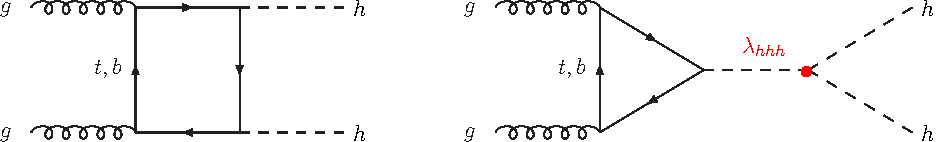
\includegraphics[width=0.9\textwidth]{Introduction/Images/dia1_hlabels_lambda_hhh.pdf}
\caption{Typical diagrams contributing to Higgs boson pair
production via gluon fusion. The contribution of the trilinear Higgs boson
self-coupling is marked in red.}
\label{fg:hhdia}
\end{center}
\end{figure}
%Higgs boson pairs are mainly produced via the gluon-fusion mechanism $gg\to hh$ which is primarily mediated by top-quark loops and receives only a small
The contribution
from bottom-quark loops is at the sub-percent level. The box diagrams (left) and the triangle diagrams (right) interfere destructively; the latter is the one sensitive to the trilinear Higgs boson self-coupling $\lambda_{hhh}$. The dependence of the cross section on the size
of the trilinear Higgs boson self-coupling can be roughly estimated as
$\Delta\sigma/\sigma \sim -\Delta\lambda_{hhh}/\lambda_{hhh}$ in the vicinity of the
SM value of $\lambda_{hhh}$. Therefore, determining the trilinear Higgs boson self-coupling
from Higgs boson pair production requires a reduction of the theoretical uncertainty on the corresponding cross section;
notably, the inclusion of
higher-order corrections becomes indispensable.

The QCD corrections were first obtained at next-to-leading order (NLO) in the heavy-top limit (HTL) \cite{Dawson:1998py}, later including the full top quark mass dependence
up to NLO \cite{Borowka:2016ehy,Borowka:2016ypz, Baglio:2018lrj,Baglio:2020ini,Baglio:2020wgt} and at next-to-next-to-leading order (NNLO) in the HTL \cite{deFlorian:2013uza,
deFlorian:2013jea, Grigo:2014jma}. Meanwhile, the next-to-next-to-next-to-leading order (N$^3$LO) QCD
corrections have been computed in the HTL,
resulting in a small further increase of the cross section
\cite{Banerjee:2018lfq, Chen:2019lzz, Chen:2019fhs, Chen:2026zmi}, as well as the N$^3$LO+N$^3$LL corrections~\cite{Ajjath:2022kpv}, where the residual scale uncertainties are at the percent level. Consequently, other theory uncertainties now play a dominant role.

The QCD corrections
increase the total LO cross section by about a factor of two. The full NLO results have been matched to parton showers \cite{Heinrich:2017kxx, Jones:2017giv,Bagnaschi:2023rbx} and the full NNLO results in the
HTL have been merged with the NLO mass effects and
supplemented by additional top quark mass effects in the double-real
corrections \cite{Grazzini:2018bsd}.
%However, a reliable estimate of the theoretical uncertainties is necessary, i.e.~considering the usual
%renormalization and factorization scale dependences but in addition also the uncertainties induced by the top-mass scheme and scale dependence.
Apart from the renormalization and factorization scale uncertainties, the following uncertainties are assessed in this report: uncertainties induced by the top quark mass scheme and scale dependence, uncertainties due to missing finite top quark mass effects and the impact of NLO electroweak corrections.


\subsection{General considerations}

The amplitude for $g(p_1) g(p_2) \to h(p_3) h(p_4)$ can be decomposed as~\cite{Glover:1987nx}\footnote{In Ref.~\cite{Bi:2023bnq}, the existence of an additional $\Delta_5$ tensor structure, containing a single Levi-Civita symbol and related to electroweak corrections, is considered. This new tensor structure plays no role at NLO since it vanishes upon contraction with the Born amplitude.}
\begin{align}
    \begin{aligned}
        \mathcal{M}_{ab}&=\delta_{ab}\,\epsilon^\mu (p_1,n_1)\epsilon^\nu (p_2,n_2)\,\mathcal{M}_{\mu\nu}   \,,\\
        \mathcal{M}^{\mu\nu}&=\frac{\alpha_s}{8\pi v^2}\left[
        F_1(\hat{s},\hat{t},m_h^2,m_t^2,D)\,T_1 ^{\mu\nu} +
        F_2(\hat{s},\hat{t},m_h^2,m_t^2,D)\,T_2 ^{\mu\nu}
        \right],
    \end{aligned}
    \label{eq:FFdeco}
\end{align}
where $m_h$ and $m_t$ are the Higgs boson and top quark masses, respectively, $D$ is the number of spacetime dimensions, $a$ and $b$ are colour indices, and the tensor structures $T_{1,2}^{\mu\nu}$ read
\begin{align}
    \begin{aligned}
        T_1^{\mu\nu} &= g^{\mu\nu} - \frac{1}{p_{12}}
        p_2^\mu p_1^\nu
        \,,\\
        T_2^{\mu\nu} &= g^{\mu\nu} + \frac{1}{p_{12} p_T^2}
    \left(
        m_h^2 p_2^\mu p_1^\nu - 2 p_{23} p_3^\mu p_1^\nu - 2 p_{13} p_2^\mu p_3^\nu + 2 p_{12} p_3^\mu p_3^\nu
    \right)
    \end{aligned}
\end{align}
with
\begin{align}
    p_T^2 = \frac{2 p_{13} p_{23}}{p_{12}} - m_h^2\quad\mbox{and}\quad p_{ij}=p_i\cdot p_j
    \,.
\end{align}
The form factors $F_{1,2}$ are related to helicity amplitudes by
\begin{align}
    \begin{aligned}
        \mathcal{M}^{++}    = \mathcal{M}^{--} &= -\frac{\alpha_s}{8\pi v^2} \,F_1(\hat{s},\hat{t},m_h^2,m_t^2,D) \,,\\
        \mathcal{M}^{+-}    = \mathcal{M}^{-+} &= -\frac{\alpha_s}{8\pi v^2} \,F_2(\hat{s},\hat{t},m_h^2,m_t^2,D)
        \,,
    \end{aligned}
\end{align}
and can be extracted by applying the projectors $P_{1,2}^{\mu\nu}$ to $\mathcal{M}^{\mu\nu}$ as
\begin{align}
    \label{eq:in:ffe}
    \begin{aligned}
        P_1^{\mu\nu} \mathcal{M}_{\mu\nu}   &= \frac{\alpha_s}{8\pi v^2}\,F_1(\hat{s},\hat{t},m_h^2,m_t^2,D)
        \,, \\
        P_2^{\mu\nu} \mathcal{M}_{\mu\nu}   &= \frac{\alpha_s}{8\pi v^2}\,F_2(\hat{s},\hat{t},m_h^2,m_t^2,D)\,,
    \end{aligned}
\end{align}
with
\begin{align}
    \begin{aligned}
        P_1^{\mu\nu}    &=
        \frac{1}{4}\frac{D-2}{D-3} T_1^{\mu\nu} - \frac{1}{4}\frac{D-4}{D-3} T_2^{\mu\nu}
        \,,\\
        P_2^{\mu\nu}    &=
        \frac{1}{4}\frac{D-2}{D-3} T_2^{\mu\nu} - \frac{1}{4}\frac{D-4}{D-3} T_1^{\mu\nu}
        \,.
    \end{aligned}
\end{align}
Higher-order corrections require the determination of both virtual and real contributions. In the latter case, extra partons have to be considered, producing new tensor structures. For QCD corrections, all possible non-zero combinations of coloured partons must be considered, while NLO EW corrections do not produce real corrections, thanks to Furry's theorem.

This report is organized as follows. Section~\ref{sec:nlo-qcd} reviews the
NLO QCD corrections with full top quark mass effects, including the matching
to parton showers and the treatment of finite top quark mass effects in the relevant
amplitudes. Section~\ref{sec:nnlo-qcd} discusses the approximate NNLO QCD
predictions, while Section~\ref{sec:n3lo-qcd} summarizes the N$^3$LO QCD
corrections and the impact of soft-gluon resummation.
Section~\ref{sec:scheme-scale-uncertainties} is devoted to the top quark mass
scheme and scale uncertainties, and Section~\ref{sec:ew-sm} reviews the
electroweak corrections in the Standard Model. The purpose of these sections
is to describe the methods and intermediate results, in some cases obtained
with choices of parameters and PDF sets that differ from those used in the
final recommendations; the definitive numbers are the recommendations collected
at the end of the report. The final cross section recommendations are presented
in Section~\ref{sec:recs}. In particular, Table~\ref{tab:final_xs_reco_125}
shows the combined final recommendation, including the dominant uncertainty
stemming from the top quark mass scheme dependence, and
Table~\ref{tab:final_xs_reco_125_mh} shows the variation of the recommended
cross section with the Higgs-boson mass. Section~\ref{subsec:mhh_distribution}
presents the recommended differential distributions for the Higgs boson pair invariant mass, $m_{hh}$.
